\chapter{Pulsos ultrarrápidos: fundamentos físicos}
\label{ch:Theoretical background}
\chapterminitoc

% ============================================================
%  CAPITULO 3 -- MARCO TEORICO
%  Seccion 3.1  ---  Propagacion de un pulso: regimen lineal y no lineal
%  (base que alimenta los operadores de la ecuacion maestra de Haus, 3.3)
% ============================================================

\section{Propagación de un pulso: régimen lineal y no lineal}
\label{sec:propagacion}

Antes de describir cómo la cavidad moldea un pulso ronda tras ronda conviene
establecer el objeto que se propaga y las dos influencias elementales que lo
transforman al atravesar cualquier medio material: la dispersión, de carácter
lineal, y la no linealidad de Kerr. Ambas reaparecerán, ya promediadas por
tránsito, como operadores de la ecuación maestra de Haus
(Sección~\ref{sec:haus}); aquí se deducen en su forma de propagación para dejar
sentado su origen físico y su notación.

\subsection{La envolvente de campo lentamente variable}

Un pulso ultracorto es una oscilación óptica de frecuencia portadora $\omega_0$
modulada por una envolvente que varía mucho más despacio que la portadora. Esta
separación de escalas justifica la \emph{aproximación de envolvente lentamente
variable}, en la que el campo eléctrico real se escribe como
%
\begin{equation}
    E(z,t) = \tfrac{1}{2}\,A(z,t)\,
    e^{\,i(k_0 z - \omega_0 t)} + \text{c.c.},
    \label{eq:envolvente}
\end{equation}
%
donde $A(z,t)$ es la envolvente compleja —cuyo módulo $|A|^2$ mide la intensidad
instantánea y cuya fase codifica la estructura de frecuencias del pulso—, $k_0$
es el número de onda a la portadora y c.c.\ denota el complejo conjugado. Toda la
dinámica de interés (ensanchamiento, \emph{chirp}, acortamiento) se traslada así a
la evolución de $A$, mucho más lenta que las oscilaciones a $\omega_0$. Describir
esa evolución es el objeto de esta sección.

\subsection{Régimen lineal: dispersión de la velocidad de grupo}

En un medio transparente, las distintas componentes espectrales del pulso viajan
con velocidades de fase diferentes porque el número de onda depende de la
frecuencia, $k=k(\omega)$. Desarrollando esta relación de dispersión en torno a la
portadora,
%
\begin{equation}
    k(\omega) = k_0 + k_1\,(\omega-\omega_0)
    + \tfrac{1}{2}\,k_2\,(\omega-\omega_0)^2 + \cdots,
    \qquad
    k_n \equiv \left.\frac{d^{\,n}k}{d\omega^{\,n}}\right|_{\omega_0},
    \label{eq:beta_expansion}
\end{equation}
%
se identifican dos coeficientes de significado físico directo. El término de
primer orden, $k_1 = 1/v_g$, es el inverso de la velocidad de grupo y no deforma
el pulso: se limita a desplazarlo en bloque. Adoptando un marco de referencia que
viaja con el pulso, $t \to t - z/v_g$, ese término se elimina y la deformación
queda gobernada por el coeficiente de segundo orden $k_2$, la \emph{dispersión de
la velocidad de grupo} (GVD). En este marco comóvil, la envolvente evoluciona
según
%
\begin{equation}
    \frac{\partial A}{\partial z}
    = i\,D_0\,\frac{\partial^2 A}{\partial t^2},
    \qquad D_0 \equiv -\tfrac{1}{2}\,k_2 ,
    \label{eq:gvd_prop}
\end{equation}
%
una ecuación de tipo Schrödinger libre cuyo efecto es puramente dispersivo: no
altera el espectro $|\tilde A(\omega)|^2$, sino que reorganiza las fases
relativas de sus componentes. El signo de $k_2$ separa dos regímenes. En
\emph{dispersión normal} ($k_2>0$, es decir $D_0<0$) las componentes de baja
frecuencia adelantan a las de alta, y el pulso adquiere un \emph{chirp} positivo
al tiempo que se ensancha temporalmente. En \emph{dispersión anómala}
($k_2<0$, $D_0>0$) ocurre lo contrario. Este segundo régimen es el relevante para
la formación de solitones, como se verá en la Sección~\ref{sec:solitones}: solo
con dispersión anómala puede la no linealidad de Kerr contrarrestar el
ensanchamiento y estabilizar el pulso.

Conviene subrayar que la GVD, por sí sola, conserva el ancho de banda del pulso y
por tanto su duración mínima alcanzable. Un pulso cuya duración temporal es la
menor compatible con su ancho espectral se denomina \emph{limitado por
transformada}; la dispersión lo aleja de ese límite introduciendo \emph{chirp},
pero una compensación dispersiva de signo opuesto puede, en principio,
restaurarlo. Esta reversibilidad distingue a la dispersión de los procesos que sí
modifican el contenido espectral, a los que se pasa a continuación.

\subsection{Régimen no lineal: efecto Kerr y automodulación de fase}

A las intensidades pico que alcanzan los pulsos ultracortos, la respuesta del
medio deja de ser lineal. El efecto Kerr óptico hace que el índice de refracción
dependa de la intensidad instantánea,
%
\begin{equation}
    n(I) = n_0 + n_2\,I,
    \qquad I \propto |A|^2,
    \label{eq:kerr}
\end{equation}
%
con $n_2>0$ el índice no lineal del material \cite{Boyd2004}. Puesto que la fase
acumulada por el campo es proporcional al índice, una envolvente de intensidad
variable imprime sobre sí misma un desfase que sigue su propio perfil temporal:
este es el fenómeno de \emph{automodulación de fase} (SPM). En términos de la
envolvente, su contribución a la propagación es
%
\begin{equation}
    \frac{\partial A}{\partial z}
    = -\,i\,\delta_0\,|A|^2 A,
    \qquad \delta_0 \propto n_2\,\omega_0 ,
    \label{eq:spm_prop}
\end{equation}
%
donde $\delta_0>0$ es el coeficiente de no linealidad. A diferencia de la GVD, la
SPM no reordena fases a espectro constante: al ser el desfase proporcional a la
intensidad, sus flancos temporales —donde $|A|^2$ varía con rapidez— generan
\emph{nuevas} componentes de frecuencia, ensanchando el espectro del pulso. Es,
por tanto, el mecanismo que permite acceder a anchos de banda —y con ellos a
duraciones— que la sola cavidad lineal no alcanzaría.

\subsection{La ecuación no lineal de Schrödinger}

Cuando dispersión y no linealidad actúan simultáneamente sobre el mismo tramo de
propagación, sus contribuciones \eqref{eq:gvd_prop} y \eqref{eq:spm_prop} se suman
y dan lugar a la \textbf{ecuación no lineal de Schrödinger} (NLSE), ecuación
canónica de la óptica de pulsos \cite{Agrawal2019}:
%
\begin{equation}
    \frac{\partial A}{\partial z}
    = i\,D_0\,\frac{\partial^2 A}{\partial t^2}
      - i\,\delta_0\,|A|^2 A .
    \label{eq:nlse}
\end{equation}
%
El signo relativo entre ambos términos es la clave de la dinámica ultrarrápida:
la GVD anómala ($D_0>0$) impone sobre el pulso un \emph{chirp} de un signo, y la
SPM ($\delta_0>0$) uno de signo opuesto. Cuando ambos se cancelan exactamente, el
pulso propaga sin deformarse —es un solitón óptico—, resultado que la
Sección~\ref{sec:solitones} desarrolla en el contexto de la cavidad. La
ecuación~\eqref{eq:nlse} describe, no obstante, un medio conservativo: no contempla
ni ganancia ni pérdidas, y admite un continuo de soluciones sin seleccionar
ninguna. Un oscilador real requiere ambos ingredientes, y es ahí donde la
descripción por propagación cede el paso a la descripción por cavidad.

\subsection{Del medio de propagación a la cavidad}

En un oscilador de bloqueo de modos el pulso no recorre un medio extenso una sola
vez, sino que atraviesa repetidamente una secuencia de elementos discretos —el
cristal de ganancia, el modulador, los espejos, los tramos de aire o de material
dispersivo— completando un circuito cerrado en cada tiempo de ida y vuelta $T_R$.
El efecto neto de la dispersión y la no linealidad sobre una ronda completa se
obtiene integrando la NLSE~\eqref{eq:nlse} a lo largo del circuito, lo que
convierte los coeficientes locales $D_0$ y $\delta_0$ en \emph{parámetros netos
por ronda}: la dispersión intracavitaria acumulada $D$ y el coeficiente de
automodulación de fase efectivo $\delta$. En esta imagen, la contribución de la
NLSE a la evolución del pulso de una vuelta a la siguiente se escribe como los dos
operadores
%
\begin{equation}
    \Delta_{D} A = i\,D\,\frac{\partial^2 A}{\partial t^2},
    \qquad
    \Delta_{\delta} A = -\,i\,\delta\,|A|^2 A ,
    \label{eq:nlse_cavidad}
\end{equation}
%
que son precisamente los términos dispersivo y no lineal de la ecuación maestra de
Haus introducidos en la Sección~\ref{sec:haus}
(ecuaciones~\eqref{eq:op_gvd} y~\eqref{eq:op_spm}). La ecuación
maestra completa la NLSE~\eqref{eq:nlse} añadiéndole justamente lo que a esta le
falta para describir un oscilador —la ganancia con ancho de banda finito, las
pérdidas lineales y el mecanismo de bloqueo de modos—, que son los términos
disipativos encargados de fijar, de entre el continuo de soluciones de la NLSE,
el pulso estacionario que el láser efectivamente emite. Con la física de la
propagación ya establecida, la siguiente sección construye esa cavidad y su
dinámica.

% ============================================================
%  CAPITULO 3 -- MARCO TEORICO
%  Seccion 3.2  ---  Bloqueo de modos: la cavidad como sistema
%                    dinamico disipativo
%  (integra y refina el borrador; alimenta la ecuacion maestra 3.3)
% ============================================================

\section{Bloqueo de modos: la cavidad como sistema dinámico disipativo}
\label{sec:mode_locking}

El bloqueo de modos (del inglés, \emph{mode-locking}) constituye la técnica
fundamental para la generación de pulsos ópticos en el régimen ultrarrápido. En un
oscilador que opera bajo bloqueo de modos en onda continua (\emph{CW
mode-locking}), la duración temporal de los pulsos emitidos es órdenes de magnitud
inferior al tiempo de ida y vuelta de la cavidad (\emph{round-trip time}), el cual
dicta de manera estricta la tasa de repetición del sistema. Típicamente, este
régimen se caracteriza por la propagación intracavidad de un único pulso
ultracorto confinado a una escala de pico\-/ o femtosegundos, o bien de un tren de
pulsos con espaciamiento temporal constante en el caso de operar bajo bloqueo de
modos armónico.

\begin{figure}[h]
    \centering
    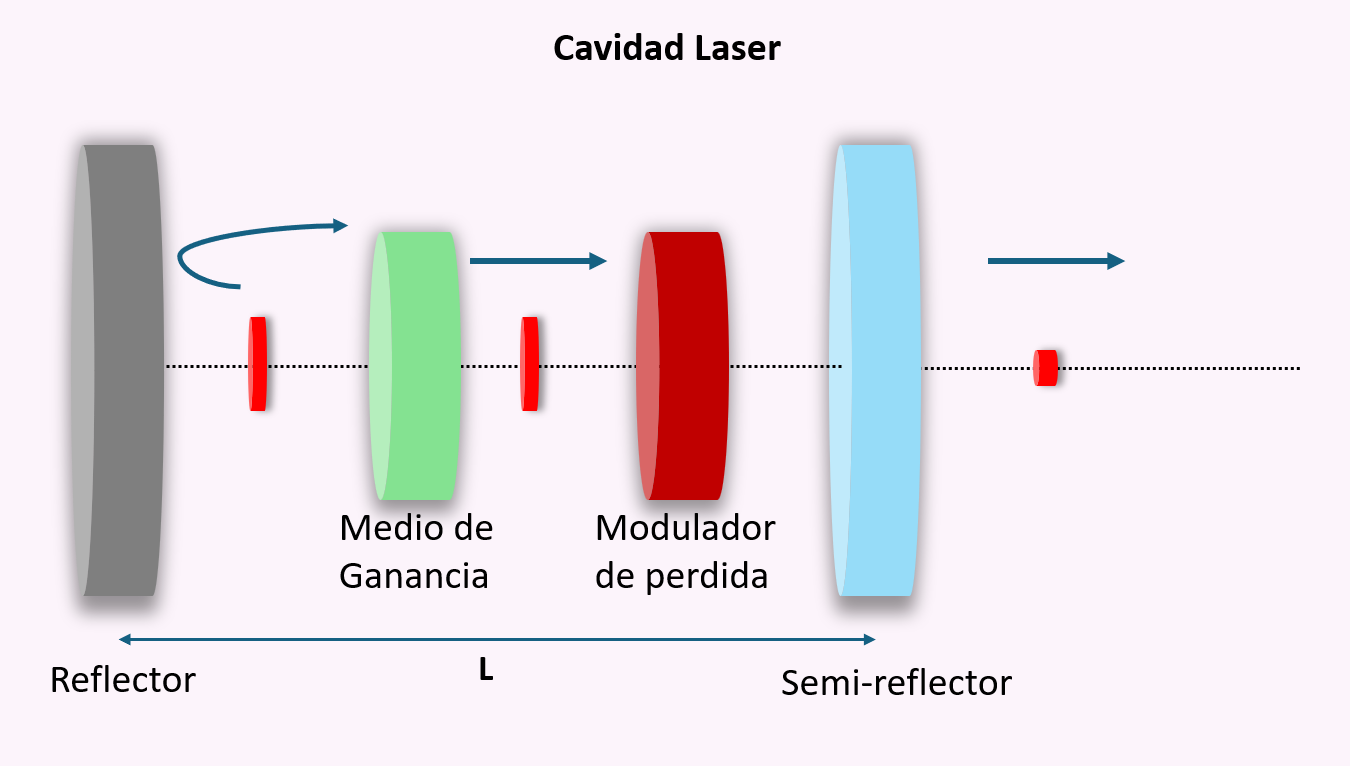
\includegraphics[scale=0.3]{chapters/images/ch3/CavidadLaser_fig3.png}
    \caption{Representación esquemática de la cavidad resonante de un láser de
    longitud $L$, diseñada para operar en régimen de bloqueo de modos. El sistema
    alberga un medio activo (ganancia) y un elemento de modulación (pérdida). La
    cavidad está delimitada por un espejo de alta reflectancia (HR) en un extremo
    y un espejo acoplador de salida semitransparente (OC) en el opuesto.}
    \label{fig:CavidadLaser_fig3}
\end{figure}

La arquitectura clásica de un láser de modos bloqueados requiere la integración de
un elemento modulador en el interior de la cavidad (véase la
Figura~\ref{fig:CavidadLaser_fig3}). La propagación del campo electromagnético a
través de este componente permite la formación de pulsos sincronizados con los
instantes de mínima atenuación impuestos por el modulador. La periodicidad
intrínseca de esta modulación coincide con el tiempo de ida y vuelta de la
cavidad, matemáticamente definido como $T_R = 2L/v_g$, donde $L$ representa la
longitud óptica de la cavidad y $v_g$ denota la velocidad de grupo del paquete de
ondas en el medio. Entender el bloqueo de modos exige, por tanto, analizar la
cavidad no como un simple amplificador resonante, sino como un \emph{sistema
dinámico disipativo}: un circuito en el que, ronda tras ronda, compiten aportes y
sustracciones de energía hasta que el pulso alcanza un estado estacionario. Las
dos subsecciones siguientes examinan primero los procesos físicos que participan
en esa competencia y después el principio de coherencia de fase que da origen al
pulso.

\subsection{Procesos inmersos en el bloqueo de modos}
\label{sec:procesos_mode_locking}

Para establecer y sostener el régimen de bloqueo de modos es imperativo incorporar
un mecanismo —moduladores activos o elementos pasivos fuertemente no lineales— que
induzca una relación de fase rígidamente coherente entre los múltiples modos
longitudinales resonantes de la cavidad. La dinámica espaciotemporal del pulso
ultracorto durante su propagación intracavidad está dictada por la interacción
altamente compleja de diversos fenómenos físicos, cada uno de los cuales
reaparecerá, promediado por ronda, como un término de la ecuación maestra de Haus
(Sección~\ref{sec:haus}):

\begin{itemize}
    \item \textbf{Ganancia.} Como en todo oscilador, se requiere un medio activo
    que provea amplificación suficiente para compensar las pérdidas totales.
    Mientras que en regímenes monomodo la ganancia es sensible exclusivamente a la
    potencia promedio, en el bloqueo de modos la elevada intensidad pico de los
    pulsos ultracortos puede inducir una saturación dinámica y rápida del medio
    activo (efecto particularmente relevante en láseres de colorante o
    semiconductores). Este agotamiento abrupto de la ganancia forma
    asimétricamente el perfil del pulso, facilitando su acortamiento temporal.

    \item \textbf{Pérdida lineal.} Engloba la atenuación no dependiente de la
    intensidad resultante de la transmisión intencionada a través del acoplador de
    salida, así como la absorción y dispersión parásitas en los componentes
    ópticos. Un diseño que optimice la relación entre ganancia y pérdidas lineales
    es insoslayable para suprimir inestabilidades del tipo \emph{Q-switching} y
    garantizar la estabilidad macroscópica del tren de pulsos.

    \item \textbf{Modulación activa.} Consiste en la introducción de un elemento
    acustoóptico o electroóptico (modulador de amplitud o de fase) impulsado por un
    sintetizador de radiofrecuencia externo. Para lograr el bloqueo de modos, la
    frecuencia de este forzamiento externo debe coincidir con la del resonador
    pasivo, induciendo bandas laterales que acoplan en fase los modos
    longitudinales adyacentes. Es el mecanismo del bloqueo de modos activo
    (Sección~\ref{sec:ml_activo}).

    \item \textbf{Pérdida saturable (modulación pasiva de amplitud).} Ocurre cuando
    la atenuación intracavidad responde de manera inversamente proporcional a la
    intensidad. Este mecanismo no lineal favorece la transmisión de las
    intensidades pico y atenúa las componentes de baja intensidad o ruido de fondo.
    Los dispositivos de pérdida saturable —tales como los espejos absorbedores
    saturables de semiconductor (SESAM) y el efecto de lente de Kerr (KLM)— se
    clasifican en «rápidos» o «lentos» en función del tiempo de relajación de sus
    portadores relativo a la duración del pulso. Es el mecanismo del bloqueo de
    modos pasivo (Sección~\ref{sec:ml_pasivo}).

    \item \textbf{Automodulación de fase (SPM).} Derivada del efecto Kerr óptico
    (Sección~\ref{sec:propagacion}), la SPM es un fenómeno paramétrico en el cual
    el índice de refracción del material depende de la intensidad lumínica
    transitoria. En osciladores ultrarrápidos su tiempo de respuesta es
    cuasi\-/instantáneo, provocando un desplazamiento de fase no lineal proporcional
    a la envolvente temporal del pulso, lo que se traduce en la generación de
    nuevas componentes frecuenciales y un severo ensanchamiento espectral.

    \item \textbf{Dispersión de la velocidad de grupo (GVD).} La dependencia de la
    velocidad de fase con la frecuencia (Sección~\ref{sec:propagacion}) provoca que
    las distintas componentes espectrales del pulso transiten por la cavidad con
    velocidades diferenciadas. En un medio de dispersión normal, esto induce un
    ensanchamiento temporal (\emph{chirping}) sistemático del pulso. Para
    contrarrestar esta deformación y preservar la coherencia temporal es imperativo
    implementar esquemas de compensación intracavidad (p.\,ej.\ pares de prismas o
    espejos fuertemente \emph{chirpeados}).

    \item \textbf{Dinámica solitónica.} Es el corolario del balance determinista
    entre la automodulación de fase y una dispersión anómala neta en la cavidad.
    Mientras la SPM genera un \emph{chirp} de frecuencia en el frente del pulso, la
    dispersión anómala lo invierte; su mutua cancelación permite la propagación de
    solitones ópticos, paquetes de onda robustos que mantienen una estructura
    temporal invariante a lo largo de miles de tránsitos
    (Sección~\ref{sec:solitones}).

    \item \textbf{Limitación del ancho de banda y filtrado pasivo.} La emisión
    sostenible en el oscilador está acotada por el ancho de banda intrínseco del
    medio de ganancia y por la reflectividad espectral de la óptica intracavidad.
    Por el principio de incertidumbre tiempo\-/ancho de banda, la duración mínima
    de un pulso ultracorto está dictada por la máxima anchura espectral que los
    elementos pasivos permitan oscilar coherentemente, lo que constituye el límite
    fundamental de la técnica.
\end{itemize}

\subsection{Principios básicos del bloqueo de modos}
\label{sec:principios_mode_locking}

La dinámica de oscilación en una cavidad láser está intrínsecamente gobernada por
las condiciones de frontera, las cuales definen los modos axiales permitidos. El
bloqueo de modos consiste en el establecimiento de una relación de fase fija y
coherente entre estos modos longitudinales. Este fenómeno se induce mediante la
incorporación de un mecanismo de modulación intracavidad que genera una
perturbación periódica en las pérdidas o en la ganancia del resonador, forzando la
oscilación simultánea y sincronizada de múltiples modos. La interferencia
constructiva resultante de este acoplamiento de fase da lugar a la formación de
pulsos ultracortos de alta intensidad, mientras que la interferencia destructiva
en las regiones inter-pulsos minimiza la emisión en el dominio temporal.

\begin{figure}[h]
    \centering
    \begin{minipage}{0.47\textwidth}
        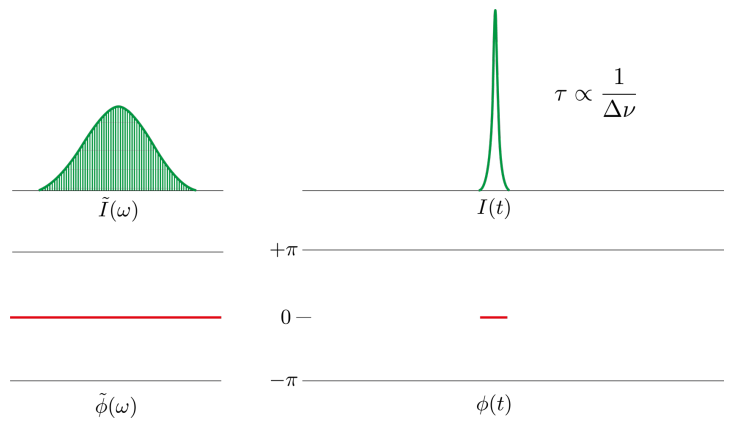
\includegraphics[width=\textwidth]{chapters/images/ch3/Modelocking_fig2a.png}
    \end{minipage}
    \hfill
    \begin{minipage}{0.47\textwidth}
        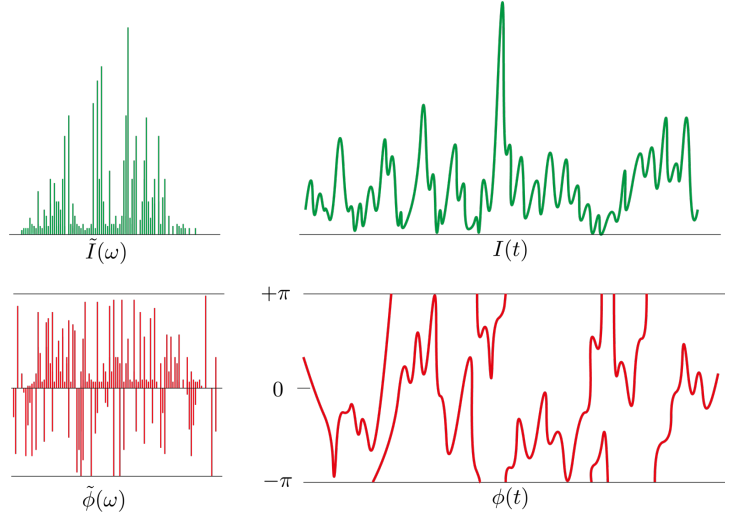
\includegraphics[width=\textwidth]{chapters/images/ch3/Modelocking_fig2b.png}
    \end{minipage}
    \caption{Caracterización del espectro óptico en función de la intensidad
    $\tilde{I}(\omega)$ y la fase $\tilde{\phi}(\omega)$. (a) Régimen de bloqueo de
    modos: la coherencia de fase entre los múltiples modos longitudinales genera un
    espectro estructurado y estable, cuya interferencia constructiva resulta en la
    formación de un pulso ultracorto en el dominio temporal. (b) Régimen de emisión
    multi-modo incoherente: la distribución estocástica de la intensidad y la fase
    en los modos axiales produce una señal temporal caracterizada por fluctuaciones
    aleatorias consistentes con ruido óptico, impidiendo la formación de una
    envolvente de pulso definida.}
    \label{fig:blockMode_CW}
\end{figure}

La duración del pulso $\tau_p$ es inversamente proporcional al número de modos
acoplados, lo que implica que un mayor ancho de banda espectral permite la
generación de pulsos temporalmente más estrechos, limitados únicamente por la
transformada de Fourier. Para un conjunto de modos axiales con un espaciamiento de
frecuencia angular constante $\Delta\omega_{ax}$, una amplitud compleja
$\tilde{E}(\omega)$ y una distribución de fase $\phi(\omega)$, el campo eléctrico
en el dominio de la frecuencia se expresa como
%
\begin{equation}
    \tilde{E}_{\text{tren}}(\omega)
    = \tilde{E}(\omega)\,e^{i\tilde{\phi}(\omega)}
      \sum_{m=-\infty}^{\infty} \delta(\omega - m\,\Delta\omega_{ax}),
    \label{eq:tren_frecuencia}
\end{equation}
%
donde $m \in \mathbb{Z}$ indexa los modos longitudinales. En el dominio espectral,
la intensidad $\tilde{I}_{\text{tren}}(\omega) = |\tilde{E}_{\text{tren}}(\omega)|^2$
se manifiesta como un peine de frecuencias. Al aplicar la transformada inversa de
Fourier a la ecuación~\eqref{eq:tren_frecuencia} se obtiene la descripción del
tren de pulsos en el dominio temporal:
%
\begin{equation}
    \begin{aligned}
        I_{\text{tren}}(t)
        &= I_p(t) \ast \sum_{m=-\infty}^{\infty}\delta(t - mT_R)\\
        &= \int_{-\infty}^{\infty} \sum_{m=-\infty}^{\infty}
           \delta(\tau - mT_R)\, I_p(t - \tau)\, d\tau\\
        &= \sum_{m=-\infty}^{\infty}
           \int_{-\infty}^{\infty} \delta(\tau - mT_R)\, I_p(t - \tau)\, d\tau\\
        &= \sum_{m=-\infty}^{\infty} I_p(t - mT_R),
    \end{aligned}
    \label{eq:tren_tiempo}
\end{equation}
%
donde se ha empleado que la transformada de Fourier de un peine de deltas produce
otro peine de deltas, y que el producto de dos funciones en el dominio espectral
equivale a la convolución de sus transformadas inversas. Este resultado ilustra
cómo el tren de pulsos en el dominio temporal es una suma de pulsos individuales
$I_p(t)$, cada uno desplazado por un múltiplo entero del periodo de repetición
$T_R$. La duración de cada pulso $I_p(t)$ viene dada por $\tau_p$, determinada por
el ancho espectral óptico $\tilde{I}(\nu)$, y con una tasa de repetición definida
como
%
\begin{equation}
    f_{\text{rep}} = \Delta\nu_{ax}
    = \frac{\Delta\omega_{ax}}{2\pi} = \frac{1}{T_R}.
    \label{eq:tasa_repeticion}
\end{equation}
%
Es imperativo distinguir entre la naturaleza espectral de un pulso aislado y la de
un tren de pulsos. Mientras que un pulso único presenta un espectro continuo, la
periodicidad intrínseca del tren impuesta por la cavidad resulta en un espectro
discreto o «peine de frecuencias». Como se ilustra en la
Figura~\ref{fig:blockMode_CW}, el bloqueo de modos transforma una emisión
multi-modo incoherente (ruido) en una estructura temporalmente localizada y
altamente estable.

\begin{figure}[h]
    \centering
    \begin{minipage}{0.47\textwidth}
        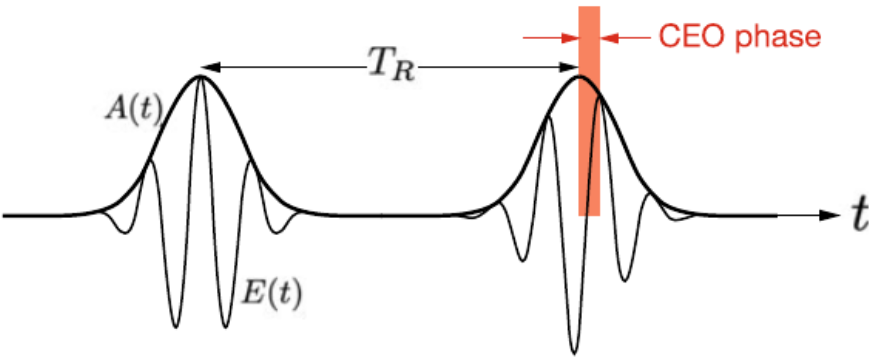
\includegraphics[width=\textwidth]{chapters/images/ch3/CEO_Phase.png}\\
        \small (a) Dominio temporal.
    \end{minipage}
    \hfill
    \begin{minipage}{0.47\textwidth}
        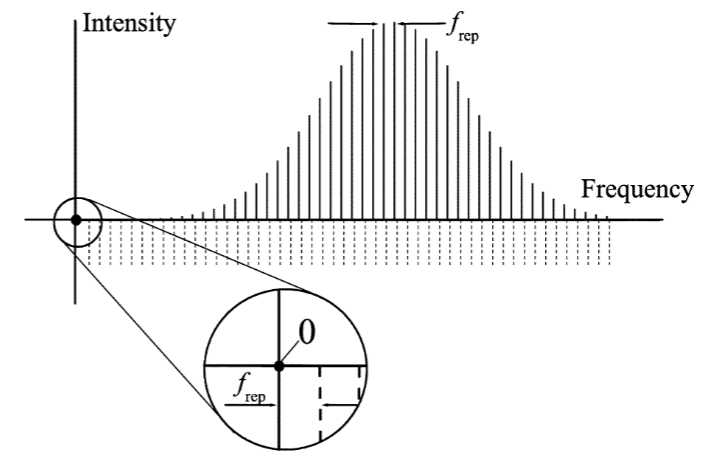
\includegraphics[width=\textwidth]{chapters/images/ch3/equidistantFrecuencyComb.png}\\
        \small (b) Dominio espectral.
    \end{minipage}
    \caption{Dinámica temporal y espectral de un tren de pulsos ultracortos.
    (a) Dominio temporal, donde se ilustra la evolución de la fase
    portadora\-/envolvente (CEO). La disparidad entre las velocidades de grupo y de
    fase en la cavidad induce un desplazamiento relativo ($\Delta\phi_{ce}$) del
    campo eléctrico respecto a la envolvente en cada periodo de repetición $T_R$
    \cite{Keller2022}. (b) Dominio espectral, que evidencia la estructura de peine
    de frecuencias ópticas. El sistema posee dos grados de libertad fundamentales:
    el intervalo entre modos ($f_{\text{rep}} = 1/T_R$) y la frecuencia de
    compensación portadora\-/envolvente ($f_{CEO}$). En condiciones de dispersión
    nula, donde las velocidades de fase y de grupo coinciden, el campo eléctrico se
    reproduce idénticamente de pulso a pulso, resultando en un espectro cuyas
    líneas son múltiplos enteros de $f_{\text{rep}}$ ($f_{CEO}=0$)
    \cite{Keller2003}.}
    \label{fig:equidistantFrecuencyComb}
\end{figure}

Para la generación de pulsos ultrarrápidos, el láser debe oscilar en tantos modos
axiales como sea posible, con una relación de fase constante entre ellos. Existen
diferentes técnicas para establecer esta condición dentro del láser; todas se
denominan «técnicas de bloqueo de modos», pues los modos que forman el peine de
frecuencias quedan bloqueados en fase con una distribución bien definida. Se
clasifican en dos categorías principales. El bloqueo de modos \emph{activo}
(Sección~\ref{sec:ml_activo}) emplea moduladores externos —acusto\-/ópticos o
electro\-/ópticos— sincronizados con $T_R$. El bloqueo de modos \emph{pasivo}
(Sección~\ref{sec:ml_pasivo}) utiliza elementos no lineales, tales como
absorbedores saturables (SESAM) o el efecto Kerr óptico, que modulan las pérdidas
en función de la intensidad instantánea, permitiendo alcanzar regímenes de
femtosegundos.

En sistemas de pocos ciclos cobra importancia un grado de libertad crítico: el
desplazamiento de fase portadora\-/envolvente (\emph{carrier-envelope phase}, CEP).
Debido a la dispersión intracavidad, la velocidad de fase y la velocidad de grupo
difieren, provocando que el máximo del campo eléctrico se desplace respecto a la
envolvente del pulso en cada tránsito. Este fenómeno se traduce en el dominio
espectral como un desplazamiento global del peine de frecuencias por una cantidad
denominada frecuencia de compensación portadora\-/envolvente, $f_{CEO}$. Así, la
frecuencia de cada diente del peine queda definida por
$f_m = m\,f_{\text{rep}} + f_{CEO}$, parámetro fundamental en metrología de
frecuencias y óptica de campo fuerte.


\section{La ecuación maestra de Haus}
\label{sec:haus}
 %
Las secciones anteriores describieron la cavidad como una sucesión de elementos
—medio de ganancia, pérdidas lineales, modulador, materiales dispersivos y no
lineales— por los que el campo transita una y otra vez. Seguir la envolvente del
pulso elemento por elemento a lo largo de los miles de tránsitos que tarda el
oscilador en estabilizarse es, sin embargo, inviable y poco esclarecedor. El
formalismo de la \emph{ecuación maestra}, introducido por
Haus \cite{Haus1975fast,Haus2000} como generalización del tratamiento de
Kuizenga y Siegman \cite{KuizengaSiegman1970}, resuelve esta dificultad con una
observación física sencilla: una vez alcanzado el régimen estacionario de bloqueo
de modos, el pulso apenas cambia de una vuelta a la siguiente. Esa pequeñez del
cambio por ronda permite sustituir la secuencia discreta de operaciones por una
única ecuación diferencial continua, que constituye el núcleo del modelado de
cavidad adoptado en esta tesis y la herramienta de la que penderán los regímenes
activo (Sección~\ref{sec:ml_activo}) y pasivo (Sección~\ref{sec:ml_pasivo}).
%
%
\subsection{El promediado por ronda}
 %
El punto de partida es la separación de dos escalas temporales. Por un lado, el
\emph{tiempo local} $t$, definido en un marco de referencia que viaja con el
pulso, resuelve la estructura interna de la envolvente (la escala de
femto\-/picosegundos). Por otro, el \emph{tiempo lento} $T$ mide la evolución de
esa envolvente a lo largo de muchos tránsitos y avanza en pasos del tiempo de ida
y vuelta $T_R$; resulta cómodo tratarlo como una variable continua, de modo que
$T = n\,T_R$ con $n$ el número de ronda. La cantidad de interés es entonces la
envolvente compleja $A(T,t)$, lentamente variable en $T$ y rápidamente
estructurada en $t$.
 
Cada elemento intracavitario $j$ produce, en un solo paso, un cambio
$\Delta_j A$ sobre la envolvente. Tras un recorrido completo, el campo acumula la
suma de todas esas contribuciones:
%
\begin{equation}
    A(T + T_R,\, t) = A(T,t) + \sum_j \Delta_j A .
    \label{eq:haus_acumulacion}
\end{equation}
%
En el régimen estacionario de bloqueo de modos, cada $\Delta_j A$ es pequeño
frente a $A$, y también lo es su suma. Bajo esta hipótesis de cambio débil por
ronda, el primer miembro de la ecuación~\eqref{eq:haus_acumulacion} admite el
desarrollo $A(T+T_R,t) \approx A(T,t) + T_R\,\partial_T A$, con lo que la
diferencia entre dos vueltas consecutivas se convierte en una derivada:
%
\begin{equation}
    T_R\,\frac{\partial A}{\partial T} = \sum_j \Delta_j A .
    \label{eq:haus_maestra_forma}
\end{equation}
%
La ecuación~\eqref{eq:haus_maestra_forma} es la forma genérica de la ecuación
maestra: traduce la dinámica discreta «vuelta a vuelta» en una evolución
continua gobernada por la acción promediada de todos los elementos de la cavidad.
Resta especificar cada operador $\Delta_j A$, lo que se hace a continuación
retomando los procesos físicos ya presentados en la
Sección~\ref{sec:procesos_mode_locking}.
 
\subsection{Operadores de los elementos intracavitarios}
 
\paragraph{Ganancia con ancho de banda finito.}
El medio activo amplifica la envolvente, pero solo dentro de su ancho de banda
$\Omega_g$. En el dominio de la frecuencia, el perfil de ganancia en torno a la
portadora se aproxima por una parábola, $g(\omega)\approx g\,(1-\omega^2/\Omega_g^2)$;
puesto que en el dominio temporal $\omega^2$ corresponde al operador
$-\partial^2/\partial t^2$, la acción de la ganancia sobre la envolvente es
%
\begin{equation}
    \Delta_{g} A = \left( g + D_g\,\frac{\partial^2}{\partial t^2} \right) A ,
    \qquad D_g \equiv \frac{g}{\Omega_g^2}.
    \label{eq:op_ganancia}
\end{equation}
%
El término $g\,A$ representa la amplificación neta y $D_g\,\partial_t^2 A$ la
\emph{dispersión de ganancia}: un filtrado que penaliza las componentes
espectrales más alejadas de la línea central y, por tanto, se opone al
acortamiento temporal del pulso. El valor saturado de $g$ queda fijado por la
energía intracavitaria a través de la condición de balance con las pérdidas.
 
\paragraph{Pérdida lineal.}
La atenuación independiente de la intensidad —transmisión por el acoplador de
salida y pérdidas parásitas— actúa como un simple factor de reducción:
%
\begin{equation}
    \Delta_{l} A = -\,l\,A .
    \label{eq:op_perdida}
\end{equation}
 
\paragraph{Dispersión de la velocidad de grupo (GVD).}
La dependencia de la velocidad de fase con la frecuencia introduce un desfase
cuadrático en el espectro que, en el dominio temporal, se escribe como
%
\begin{equation}
    \Delta_{D} A = i D\,\frac{\partial^2}{\partial t^2}\,A ,
    \label{eq:op_gvd}
\end{equation}
%
donde $D$ es la dispersión neta por ronda. El carácter imaginario del operador
distingue la GVD de la dispersión de ganancia: aquella reordena las fases
espectrales sin atenuar, esta filtra amplitudes.
 
\paragraph{Automodulación de fase (SPM).}
El efecto Kerr hace que el índice de refracción dependa de la intensidad
instantánea, imprimiendo sobre la envolvente un desfase no lineal proporcional a
$|A|^2$:
%
\begin{equation}
    \Delta_{\delta} A = -\,i\,\delta\,|A|^2 A ,
    \label{eq:op_spm}
\end{equation}
%
con $\delta$ el coeficiente de no linealidad por ronda. Junto con la GVD, este es
el término responsable de la dinámica solitónica que se analiza en la
Sección~\ref{sec:solitones}.
 
\paragraph{Mecanismo de bloqueo de modos.}
El elemento que sostiene el régimen pulsado se describe con un operador
$\Delta_{\mathrm{ML}}A$ cuya forma concreta depende de la técnica empleada. En el
bloqueo de modos \emph{activo}, un modulador de amplitud impone una pérdida
periódica sincronizada con la cavidad,
%
\begin{equation}
    \Delta_{\mathrm{ML}}^{\text{act}} A = -\,M\bigl(1-\cos\omega_m t\bigr)\,A ,
    \label{eq:op_modulador}
\end{equation}
%
con $M$ la profundidad de modulación y $\omega_m$ su frecuencia, igual a la de
repetición de la cavidad. En el bloqueo de modos \emph{pasivo}, un absorbente
saturable atenúa selectivamente las componentes de baja intensidad,
%
\begin{equation}
    \Delta_{\mathrm{ML}}^{\text{pas}} A = -\,q\!\left(|A|^2\right) A ,
    \label{eq:op_absorbente}
\end{equation}
%
donde $q(|A|^2)$ es una pérdida decreciente con la intensidad; para un absorbente
rápido admite la linealización $q(|A|^2)\approx q_0-\gamma|A|^2$, de modo que el
término favorece la transmisión de los picos de mayor intensidad. Las
Secciones~\ref{sec:ml_activo} y~\ref{sec:ml_pasivo} desarrollan, respectivamente,
cada una de estas dos variantes.
 
\subsection{Forma general y especializaciones}
 
Sustituyendo los operadores
\eqref{eq:op_ganancia}--\eqref{eq:op_absorbente} en la
forma genérica~\eqref{eq:haus_maestra_forma} se obtiene la \textbf{ecuación
maestra de Haus} en su versión general, que reúne en una sola expresión la
amplificación, las pérdidas, el filtrado de ganancia, la dispersión, la no
linealidad y el mecanismo de bloqueo de modos:
%
\begin{equation}
    T_R\,\frac{\partial A}{\partial T}
    = \Bigl[\,(g-l)
      + \bigl(D_g + iD\bigr)\frac{\partial^2}{\partial t^2}
      - i\,\delta\,|A|^2
      + \Delta_{\mathrm{ML}} \,\Bigr] A ,
    \label{eq:haus_general}
\end{equation}
%
con $\Delta_{\mathrm{ML}}$ dado por la
ecuación~\eqref{eq:op_modulador} en el caso activo o
por~\eqref{eq:op_absorbente} en el pasivo. La
ecuación~\eqref{eq:haus_general} es la pieza central del marco de cavidad: todas
las especializaciones que siguen en este capítulo se obtienen seleccionando qué
términos se conservan y cuáles resultan despreciables en cada régimen.
 
La condición de operación estacionaria se impone exigiendo que el pulso se
reproduzca a sí mismo de una vuelta a la siguiente, salvo un eventual
desplazamiento de fase global $\phi_0$ por ronda. Equivale a buscar soluciones de
la forma $A(T,t)=A(t)\,\exp(i\phi_0\,T/T_R)$, para las que la
ecuación~\eqref{eq:haus_general} se reduce a un problema de autovalores en el
tiempo local:
%
\begin{equation}
    i\,\phi_0\,A
    = \Bigl[\,(g-l)
      + \bigl(D_g + iD\bigr)\frac{\partial^2}{\partial t^2}
      - i\,\delta\,|A|^2
      + \Delta_{\mathrm{ML}} \,\Bigr] A .
    \label{eq:haus_estacionario}
\end{equation}
 
\paragraph{Límite de Kuizenga--Siegman.}
El caso históricamente primero —y la base sobre la que se construye el régimen
solitónico de la Sección~\ref{sec:ml_activo}— corresponde al bloqueo de modos
activo sin dispersión ni no linealidad ($D=\delta=0$). La ecuación maestra se
reduce entonces a
%
\begin{equation}
    T_R\,\frac{\partial A}{\partial T}
    = \Bigl[\,(g-l)
      + D_g\,\frac{\partial^2}{\partial t^2}
      - M\bigl(1-\cos\omega_m t\bigr) \,\Bigr] A .
    \label{eq:haus_activo_base}
\end{equation}
%
Dado que el pulso es mucho más corto que el periodo de modulación, basta
desarrollar el modulador en torno a su mínimo de pérdida,
$M(1-\cos\omega_m t)\approx M_s\,t^2$ con $M_s\equiv M\omega_m^2/2$, lo que
convierte~\eqref{eq:haus_activo_base} en la ecuación de un oscilador armónico
cuántico: sus soluciones estacionarias son funciones de Hermite--Gauss y el modo
fundamental es un pulso gaussiano cuya anchura fija el balance entre la dispersión
de ganancia $D_g$ (que lo ensancha) y la curvatura del modulador $M_s$ (que lo
estrecha). Esta es la solución de Kuizenga--Siegman \cite{KuizengaSiegman1970},
que la Sección~\ref{sec:ml_activo} retoma para incorporar después los términos de
SPM y GVD y obtener el solitón.
 
\subsection{Conexión con la ecuación no lineal de Schrödinger}
 
La forma general~\eqref{eq:haus_general} ilumina la relación entre el oscilador y
los sistemas no lineales conservativos. Si se agrupan los términos puramente
dispersivos y no lineales, el contenido entre corchetes de
la~\eqref{eq:haus_general} contiene la combinación
$iD\,\partial_t^2 A - i\delta|A|^2 A$, que es exactamente el segundo miembro de la
\textbf{ecuación no lineal de Schrödinger} (NLSE) introducida en la
Sección~\ref{sec:propagacion}. Los términos restantes —ganancia, pérdida,
dispersión de ganancia y modulación— son los que distinguen una \emph{cavidad}
de un medio conservativo: aportan y disipan energía, y seleccionan una solución
estacionaria de entre el continuo de soluciones de la NLSE. Cuando la dispersión
de ganancia y la modulación son débiles frente al balance dispersión--no
linealidad, la dinámica de~\eqref{eq:haus_general} queda dominada por su parte
NLSE y el pulso estacionario es un solitón ligeramente perturbado; cuando, por el
contrario, dominan ganancia y modulación, se recupera el régimen gaussiano de
Kuizenga--Siegman. La ecuación maestra de Haus interpola así entre ambos límites
y proporciona el marco unificado —válido para bloqueo de modos activo y pasivo—
sobre el que se asienta el resto de este capítulo \cite{Haus2000,Keller2022}.


% ============================================================
%  CAPITULO 3 -- MARCO TEORICO
%  Seccion 3.4  ---  Bloqueo de modos activo
%  (rehecha desde cero: mecanismo -> solucion de Kuizenga-Siegman
%   -> regimen solitonico; se apoya en la ecuacion maestra 3.3)
% ============================================================

\section{Bloqueo de modos activo}
\label{sec:ml_activo}

El bloqueo de modos activo es una de las primeras técnicas desarrolladas para
generar pulsos ultracortos \cite{KuizengaSiegman1970,Haus1975forced}. Consiste en
introducir en la cavidad un modulador —acusto\-/óptico o electro\-/óptico— que
modula periódicamente las pérdidas (modulación de amplitud, AM) o la fase
(modulación de frecuencia, FM) del resonador. Para que el mecanismo bloquee los
modos, la frecuencia del forzamiento externo $\omega_m$ debe coincidir con la
frecuencia de repetición de la cavidad, de modo que la modulación induce bandas
laterales que acoplan en fase los modos longitudinales adyacentes. En el dominio
temporal la imagen es más intuitiva: el modulador abre una «ventana» de mínima
pérdida una vez por tiempo de ida y vuelta $T_R$, y solo la luz que atraviesa el
elemento en ese instante sobrevive tránsito tras tránsito. La radiación es así
recortada repetidamente hasta que se concentra en un pulso sincronizado con la
ventana de transmisión, cada vez más corto, hasta que un mecanismo de
ensanchamiento detiene el proceso y fija el estado estacionario.

\subsection{Solución de Kuizenga--Siegman: el pulso gaussiano}
\label{sec:kuizenga_siegman}

El punto de partida es la ecuación maestra para el bloqueo de modos activo sin
dispersión ni no linealidad, deducida en la Sección~\ref{sec:haus}
(ecuación~\eqref{eq:haus_activo_base}). Puesto que el pulso es mucho más corto que
el periodo de modulación $2\pi/\omega_m$, basta desarrollar el modulador en torno
a su mínimo de pérdida, $M\bigl(1-\cos\omega_m t\bigr)\approx M_s\,t^2$ con
$M_s\equiv M\omega_m^2/2$. En estado estacionario ($\partial_T A = 0$) la ecuación
maestra se reduce al problema de autovalores
%
\begin{equation}
    D_g\,\frac{\partial^2 A}{\partial t^2}
    - M_s\,t^2\,A + (g-l)\,A = 0,
    \label{eq:ks_autovalores}
\end{equation}
%
formalmente idéntico al del oscilador armónico cuántico. Su modo fundamental es un
pulso de perfil gaussiano,
%
\begin{equation}
    A(t) = A_0\,\exp\!\left(-\frac{t^2}{2\tau_g^{2}}\right),
    \qquad
    \tau_g = \left(\frac{D_g}{M_s}\right)^{1/4},
    \label{eq:ks_gaussiano}
\end{equation}
%
cuya anchura resulta del equilibrio entre los dos términos que compiten en
\eqref{eq:ks_autovalores}: la dispersión de ganancia $D_g=g/\Omega_g^2$, que
ensancha el pulso al filtrar sus alas espectrales, y la curvatura del modulador
$M_s$, que lo estrecha al penalizar sus alas temporales. Sustituyendo
\eqref{eq:ks_gaussiano} en \eqref{eq:ks_autovalores} se obtiene además la
condición de balance que fija la ganancia saturada,
%
\begin{equation}
    g - l = \sqrt{D_g\,M_s},
    \label{eq:ks_balance}
\end{equation}
%
es decir, el exceso de ganancia sobre las pérdidas lineales necesario para
sostener el pulso estacionario. Expresada como anchura a media altura de la
intensidad, la duración del pulso gaussiano es
%
\begin{equation}
    \tau_p = 1.665\,\left(\frac{D_g}{M_s}\right)^{1/4}
           = 1.665\,\left(\frac{2\,D_g}{M\,\omega_m^{2}}\right)^{1/4}.
    \label{eq:tau_gauss}
\end{equation}
%
La ecuación~\eqref{eq:tau_gauss} encierra la limitación esencial del bloqueo de
modos activo puro: la duración decrece solo como la \emph{raíz cuarta} del
cociente $D_g/M_s$. Acortar el pulso a la mitad exigiría aumentar dieciséis veces
la intensidad de modulación o el ancho de banda de ganancia, lo que en la práctica
confina esta técnica al régimen de picosegundos. Alcanzar los femtosegundos
requiere un mecanismo de acortamiento más eficiente que la modulación externa; ese
mecanismo lo proporciona la interacción entre automodulación de fase y dispersión,
que da lugar al régimen solitónico.

\subsection{Pulsos solitónicos en régimen activo}
\label{sec:ml_activo_soliton}

Cuando la cavidad presenta dispersión y no linealidad apreciables, a los términos
de \eqref{eq:haus_activo_base} se añaden los operadores de GVD y SPM introducidos
en las ecuaciones~\eqref{eq:op_gvd} y~\eqref{eq:op_spm}. La ecuación maestra de
Haus para el bloqueo de modos activo en presencia de estos efectos se escribe
entonces como
%
\begin{equation}
    T_R\,\frac{\partial A}{\partial T}
    = \Bigl[\,iD\,\frac{\partial^2}{\partial t^2} - i\delta\,|A|^2 \,\Bigr] A
    + \Bigl[\,g - l + D_g\,\frac{\partial^2}{\partial t^2}
      - M\bigl(1-\cos\omega_m t\bigr) \,\Bigr] A = 0.
    \label{eq:haus_soliton}
\end{equation}
%
El primer corchete de la ecuación~\eqref{eq:haus_soliton} es la ecuación no lineal
de Schrödinger (Sección~\ref{sec:propagacion}, ecuación~\eqref{eq:nlse}), cuya
solución para dispersión anómala ($D>0$) y no linealidad focalizante es el solitón
fundamental. Dos observaciones permiten tratar el segundo corchete como una
perturbación. Por un lado, los medios de ganancia con ancho de banda suficiente
para sostener pulsos ultracortos cumplen $D_g=g/\Omega_g^2\ll 1$. Por otro, el
modulador de pérdida sinusoidal varía muy lentamente frente a la duración del
pulso, por lo que apenas actúa sobre su forma. En consecuencia, la dinámica queda
gobernada por la parte NLSE, mientras que ganancia, pérdida y modulación
desempeñan un papel perturbativo que estabiliza y selecciona la solución. La
resolución se aborda mediante teoría de perturbaciones solitónicas, sustituyendo
el perfil gaussiano de Kuizenga--Siegman por una secante hiperbólica.

Se propone así un \emph{ansatz} que describe un solitón acompañado de un fondo
residual —el continuo—,
%
\begin{equation}
    A(T,t) = A_0\,\operatorname{sech}\!\left(\frac{t}{\tau}\right)
    \exp\!\left(i\phi_0\,\frac{T}{T_R}\right) + \text{continuo},
    \label{eq:ansatz_soliton}
\end{equation}
%
donde $A_0$ es la amplitud de la envolvente, $\tau$ su duración y $\phi_0$ el
desplazamiento de fase que el solitón acumula por cada periodo de repetición
$T_R$. Con dispersión anómala suficiente, el continuo decae exponencialmente y,
para una energía de pulso dada, se forma un solitón cuya duración ideal es
%
\begin{equation}
    \tau = \frac{4\,|D|}{F_{P,L}\,\delta},
    \label{eq:tau_soliton}
\end{equation}
%
con $\delta$ el coeficiente de SPM y $F_{P,L}$ la densidad de energía del pulso en
el medio láser, bajo el supuesto de que la SPM se genera en el cristal de
ganancia. La dispersión neta por ronda $D$ se relaciona con la dispersión de
retardo de grupo acumulada mediante $\mathrm{GDD}=-2D$, de modo que el régimen
anómalo ($\mathrm{GDD}<0$) corresponde, coherentemente con la
Sección~\ref{sec:propagacion}, a $D>0$. La ecuación~\eqref{eq:tau_soliton} indica
que reducir la dispersión acorta el solitón; sin embargo, como se verá, existe un
límite por debajo del cual el pulso se desestabiliza.

\paragraph{El continuo y su papel estabilizador.}
El solitón no se forma de manera instantánea. Partiendo de un pulso gaussiano
inicial, el sistema requiere del orden de un centenar de tránsitos para relajar
hacia el estado estacionario solitónico, de duración mucho menor. La fracción de
energía del pulso inicial que no logra ajustarse al perfil del solitón se vierte
en el continuo: una componente de baja intensidad para la cual la SPM es
insuficiente para compensar el ensanchamiento dispersivo, de modo que se dispersa
temporalmente. Al ensancharse, el continuo pasa más tiempo fuera de la ventana de
transmisión del modulador y sufre en él una pérdida creciente, por lo que decae
con las rondas (Figura~\ref{fig:saturable_gain}). En el marco de referencia del
solitón, el efecto Kerr le imprime un desplazamiento de fase periódico que genera
interferencias con el continuo; estas se desvanecen gradualmente a medida que el
continuo se extingue, dejando únicamente el solitón.

\begin{figure}[h]
    \centering
    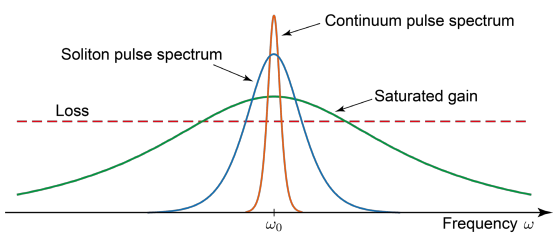
\includegraphics[width=0.8\linewidth]{chapters/images/ch3/saturable_gain.png}
    \caption{La ganancia se satura por acción del solitón. Como el continuo ocupa
    un ancho espectral menor, experimenta una ganancia efectiva mayor y tendería a
    crecer; la pérdida adicional que introduce el modulador sobre el continuo
    —temporalmente ensanchado— compensa ese exceso y previene la inestabilidad del
    solitón.}
    \label{fig:saturable_gain}
\end{figure}

\paragraph{Duración mínima y factor de reducción.}
Existe un límite a cuánto puede acortarse el solitón manteniéndolo estable frente
al continuo: si la dispersión es demasiado baja, el continuo no se ensancha con la
rapidez suficiente para ser absorbido por el modulador y el sistema se
desestabiliza, llegando a generar pulsos satélite tras muchos miles de tránsitos.
La teoría perturbativa de solitones fija ese umbral a través de la dispersión
normalizada mínima
%
\begin{equation}
    D_{n,\min} = \frac{|D|}{D_g}
    = \frac{2}{9}\sqrt[3]{\frac{(9\phi_0/2)^2}{D_g\,M_s}},
    \label{eq:disp_min}
\end{equation}
%
a la que corresponde una duración a media altura de la intensidad
%
\begin{equation}
    \tau_{\min} = 1.763\,\sqrt[3]{\frac{2\,D_g^{2}}{9\,\phi_0\,M_s}}.
    \label{eq:tau_min}
\end{equation}
%
Comparando la duración mínima solitónica~\eqref{eq:tau_min} con la del pulso
gaussiano puramente activo~\eqref{eq:tau_gauss}, el factor de reducción que aporta
el régimen solitónico es
%
\begin{equation}
    R_{\max} = \frac{\tau_p}{\tau_{\min}}
    = \frac{1.665}{1.763}\,\sqrt[12]{\frac{(9\phi_0/2)^2}{D_g\,M_s}}
    = \frac{1.665}{1.763}\,\sqrt[4]{\tfrac{9}{2}\,D_{n,\min}}.
    \label{eq:factor_reduccion}
\end{equation}
%
A diferencia del caso puramente activo, la envolvente estacionaria ya no es un
pulso gaussiano con \emph{chirp}, sino un solitón $\operatorname{sech}^2$ sin
\emph{chirp}, que es lo que permite descender al régimen de femtosegundos.

\paragraph{Balance de energía y estabilidad.}
El solitón permanece estable mientras su pérdida efectiva $l_s$ sea inferior a la
que sufre el continuo $l_c$. La pérdida del solitón consta de dos aportaciones,
%
\begin{equation}
    l_s = \frac{D_g}{3\,\tau^2}
        + \frac{\pi^2}{24}\,M\,\omega_m^2\,\tau^2,
    \label{eq:perdida_soliton}
\end{equation}
%
la primera debida al ancho de banda finito de la ganancia —que tiende a ensanchar
el solitón— y la segunda a la acción residual del modulador de pérdida. El balance
de ganancia y pérdidas se escribe entonces como $g = l + l_s$, con $l$ la pérdida
aportada por el resto de los elementos de la cavidad. Para solitones muy cortos, el
primer término domina y la influencia del modulador sobre el solitón resulta casi
nula; el continuo, en cambio, sí experimenta en el modulador una pérdida intensa,
lo que garantiza su supresión y, con ella, la estabilidad del pulso solitónico.
Este contraste entre la escasa pérdida del solitón y la elevada del continuo es,
en última instancia, el mecanismo que sostiene el bloqueo de modos activo en su
régimen solitónico \cite{Haus2000,Keller2022}.


% ============================================================
%  CAPITULO 3 -- MARCO TEORICO
%  Seccion 3.5  ---  Bloqueo de modos pasivo
%  (nueva; construida en paralelo a 3.4, cierra el par activo/pasivo)
% ============================================================

\section{Bloqueo de modos pasivo}
\label{sec:ml_pasivo}

En el bloqueo de modos activo la ventana de baja pérdida la abre un modulador
externo sincronizado con la cavidad; su rapidez está acotada por la electrónica de
radiofrecuencia y, con ella, la duración mínima del pulso queda confinada al
régimen de picosegundos (Sección~\ref{sec:ml_activo}). El bloqueo de modos
\emph{pasivo} elimina esa limitación con una idea distinta: en lugar de imponer la
modulación desde fuera, se hace que sea el propio pulso quien la genere. Un
elemento no lineal cuya pérdida disminuye al aumentar la intensidad convierte al
oscilador en un sistema que se automodula, de modo que la «ventana» de
transmisión es tan breve como el pulso mismo y se estrecha a la par que este. Por
esta razón el bloqueo de modos pasivo es la vía habitual hacia el régimen de
femtosegundos y el mecanismo dominante en la literatura de osciladores
ultrarrápidos, lo que a su vez motiva —por contraste— el interés de estudiar
también el régimen activo en el análisis comparativo de esta tesis.

\subsection{El absorbente saturable}
\label{sec:absorbente}

El componente central del bloqueo de modos pasivo es el \emph{absorbente
saturable}: un medio cuya absorción se satura a alta intensidad, de manera que su
pérdida es una función decreciente de $|A|^2$,
%
\begin{equation}
    q\!\left(|A|^2\right) = \frac{q_0}{\,1 + |A|^2/I_A\,},
    \label{eq:absorbente_general}
\end{equation}
%
donde $q_0$ es la pérdida no saturada e $I_A$ la intensidad de saturación. Frente a
un pulso, el absorbente atenúa intensamente las alas de baja intensidad y el ruido
de fondo, pero se vuelve casi transparente en el pico: cada tránsito recorta las
colas del pulso y refuerza su centro, produciendo un acortamiento neto. Este efecto
se denomina \emph{automodulación de amplitud}, y es el análogo no lineal de la
modulación activa, con una diferencia esencial: el término que introduce en la
ecuación maestra es \emph{real}, pues modula la amplitud del campo —a diferencia
de la automodulación de fase (SPM), de carácter imaginario, que modula su fase
(Sección~\ref{sec:propagacion})—.

Para un pulso cuya intensidad de pico no satura por completo el absorbente, la
respuesta~\eqref{eq:absorbente_general} admite la linealización
$q(|A|^2)\approx q_0-\gamma\,|A|^2$, con $\gamma = q_0/I_A$ el coeficiente de
automodulación de amplitud. La contribución del absorbente a la evolución del pulso
—el operador $\Delta_{\mathrm{ML}}^{\text{pas}}A$ introducido en la
Sección~\ref{sec:haus}, ecuación~\eqref{eq:op_absorbente}— se descompone entonces
en una pérdida constante $-q_0 A$, absorbible en la pérdida lineal $l$, y un
término no lineal $+\gamma|A|^2A$ que favorece las intensidades altas:
%
\begin{equation}
    \Delta_{\mathrm{ML}}^{\text{pas}} A
    = -\,q\!\left(|A|^2\right) A
    \;\approx\; -\,q_0\,A + \gamma\,|A|^2 A .
    \label{eq:op_absorbente_rapido}
\end{equation}

\subsection{Absorbente rápido y absorbente lento}
\label{sec:absorbente_tipos}

El comportamiento del absorbente depende de la relación entre su tiempo de
relajación $\tau_A$ —el que tardan sus portadores excitados en regresar al estado
fundamental— y la duración del pulso $\tau_p$. Se distinguen dos regímenes. En el
\emph{absorbente rápido} ($\tau_A \ll \tau_p$) la respuesta es prácticamente
instantánea: la pérdida sigue punto a punto el perfil de intensidad
$|A(t)|^2$ y, en consecuencia, conforma de manera simétrica ambos flancos del
pulso; es el caso descrito por la linealización~\eqref{eq:op_absorbente_rapido} y
el más favorable para alcanzar duraciones de femtosegundos. En el \emph{absorbente
lento} ($\tau_A \gg \tau_p$) el elemento se satura con el frente del pulso y se
recupera despacio, por lo que recorta eficazmente el flanco de subida pero no el de
bajada; el cierre de la ventana en la cola requiere entonces la ayuda de la
saturación dinámica de la ganancia, que agota la amplificación tras el paso del
pico. Ambos mecanismos conducen a un pulso estable, pero por caminos distintos.

\subsection{Implementaciones físicas: SESAM y KLM}
\label{sec:sesam_klm}

Dos realizaciones dominan la práctica experimental. La primera es el \emph{espejo
absorbente saturable de semiconductor} (SESAM), un absorbente real integrado en un
espejo de la cavidad, cuya absorción, intensidad de saturación y tiempo de
relajación pueden ajustarse por diseño de la estructura semiconductora. El SESAM
proporciona un arranque fiable del bloqueo de modos (\emph{self-starting}) y ha
hecho del régimen pasivo una tecnología robusta y reproducible
\cite{Keller1996,Keller2003}. La segunda es el bloqueo de modos por \emph{lente de
Kerr} (KLM), un absorbente \emph{artificial} que no descansa en ninguna absorción
real: el autoenfocamiento por efecto Kerr hace que el haz más intenso se focalice
más y, combinado con una apertura efectiva en la cavidad, sufra menos pérdida que
el fondo de baja intensidad. Al basarse en el efecto Kerr, la respuesta del KLM es
esencialmente instantánea —un absorbente rápido ideal— y es el mecanismo que ha
permitido generar los pulsos de pocos ciclos en osciladores de Ti:zafiro
\cite{Krausz1992,Keller2022}.

\subsection{Ecuación maestra del bloqueo de modos pasivo}
\label{sec:haus_pasivo}

Sustituyendo el operador del absorbente rápido~\eqref{eq:op_absorbente_rapido} en
la ecuación maestra general de Haus (Sección~\ref{sec:haus},
ecuación~\eqref{eq:haus_general}) y considerando, por simplicidad, el caso sin
dispersión ni SPM netas, la condición estacionaria toma la forma
%
\begin{equation}
    \Bigl[\,g - l + D_g\,\frac{\partial^2}{\partial t^2}
      + \gamma\,|A|^2 \,\Bigr] A = 0,
    \label{eq:haus_pasivo}
\end{equation}
%
donde la pérdida no saturada $q_0$ se ha absorbido en $l$. La
ecuación~\eqref{eq:haus_pasivo} es formalmente análoga a la del régimen activo
\eqref{eq:ks_autovalores}, pero con una diferencia decisiva: el término de
conformado, $\gamma|A|^2$, depende de la intensidad del propio pulso en lugar de la
curvatura fija $-M_s t^2$ de un modulador externo. Su solución estacionaria es un
pulso de secante hiperbólica sin \emph{chirp},
%
\begin{equation}
    A(t) = A_0\,\operatorname{sech}\!\left(\frac{t}{\tau}\right),
    \label{eq:pasivo_sech}
\end{equation}
%
cuya duración se obtiene, al sustituir~\eqref{eq:pasivo_sech}
en~\eqref{eq:haus_pasivo} e igualar por separado los términos proporcionales a
$\operatorname{sech}$ y a $\operatorname{sech}^3$, del balance entre la dispersión
de ganancia —que ensancha— y la automodulación de amplitud —que estrecha—:
%
\begin{equation}
    \tau = \frac{1}{A_0}\sqrt{\frac{2\,D_g}{\gamma}},
    \qquad\text{con}\qquad
    g - l = -\,\frac{D_g}{\tau^2}.
    \label{eq:tau_pasivo}
\end{equation}

El contraste con el bloqueo de modos activo es esclarecedor. Allí, la duración del
pulso gaussiano~\eqref{eq:tau_gauss} escalaba como $(D_g/M_s)^{1/4}$ y era
\emph{independiente} de la energía del pulso, fijada por completo por el modulador
externo. Aquí, en cambio, la duración~\eqref{eq:tau_pasivo} es
\emph{inversamente proporcional} a la amplitud $A_0$: cuanto más intenso es el
pulso, más corto se hace, en un proceso de realimentación que se refuerza a sí
mismo hasta que interviene un mecanismo limitante (el ancho de banda de ganancia, o
la propia saturación del absorbente). El absorbente saturable se comporta, en
efecto, como un modulador ideal cuya ventana de transmisión es tan breve como el
pulso y lo sigue automáticamente, algo inalcanzable para cualquier modulador
externo. Esta es la razón física por la que el bloqueo de modos pasivo accede al
régimen de femtosegundos donde el activo se detiene en los picosegundos.

Finalmente, al igual que en el caso activo, la incorporación de dispersión anómala
y SPM a la ecuación~\eqref{eq:haus_pasivo} conduce a un régimen de bloqueo de modos
solitónico, en el que la forma del pulso la fija el balance dispersión\-/no
linealidad y el absorbente se limita a estabilizarlo y a suprimir el continuo. Ese
solitón disipativo —común a ambos mecanismos de bloqueo— es el objeto de la
Sección~\ref{sec:solitones}.


% ============================================================
%  CAPITULO 3 -- MARCO TEORICO
%  Seccion 3.6  ---  Solitones y solitones disipativos
%  (cierra la Parte I; puente hacia el espacio de parametros 3.7)
% ============================================================

\section{Solitones y solitones disipativos}
\label{sec:solitones}

El solitón ha aparecido ya como la solución estacionaria a la que convergen tanto
el bloqueo de modos activo (Sección~\ref{sec:ml_activo}) como el pasivo
(Sección~\ref{sec:ml_pasivo}) cuando la cavidad presenta dispersión y no
linealidad. Esta sección consolida ese concepto en dos pasos: primero el solitón
\emph{conservativo} de la ecuación no lineal de Schrödinger, que fija la forma del
pulso, y después el solitón \emph{disipativo} propio de la cavidad, que además fija
su energía. Con ello se llega al mapa de regímenes de operación del oscilador, cuya
multiplicidad es la raíz de la dificultad que la segunda parte del capítulo
—dedicada a la optimización— busca resolver.

\subsection{El solitón fundamental de la ecuación no lineal de Schrödinger}
\label{sec:soliton_fundamental}

En un medio conservativo, sin ganancia ni pérdidas, la evolución del pulso obedece
a la ecuación no lineal de Schrödinger deducida en la
Sección~\ref{sec:propagacion} (ecuación~\eqref{eq:nlse}). Su solución más notable
resulta del equilibrio exacto entre los dos efectos que la componen: la dispersión
anómala, que introduce un \emph{chirp} sobre el pulso, y la automodulación de fase,
que introduce el \emph{chirp} opuesto. Cuando ambos se compensan punto a punto, el
pulso se propaga sin deformarse. Este pulso invariante es el \emph{solitón
fundamental}, de perfil secante hiperbólico,
%
\begin{equation}
    A(z,t) = A_0\,\operatorname{sech}\!\left(\frac{t}{\tau}\right)
    e^{\,i\kappa z},
    \label{eq:soliton_fundamental}
\end{equation}
%
que al sustituirse en la NLSE~\eqref{eq:nlse} impone una relación fija entre su
amplitud de pico $A_0$, su duración $\tau$ y los parámetros del medio —la condición
conocida como \emph{teorema del área} del solitón—,
%
\begin{equation}
    \delta_0\,A_0^{2} = \frac{2\,D_0}{\tau^{2}},
    \qquad\text{equivalentemente}\qquad
    A_0^{2}\,\tau^{2} = \frac{2\,D_0}{\delta_0},
    \label{eq:area_soliton}
\end{equation}
%
con $\kappa = D_0/\tau^2$ el desplazamiento de fase por unidad de longitud. La
ecuación~\eqref{eq:area_soliton} expresa el rasgo distintivo del solitón: cuanto
más intenso es (mayor $A_0$), más corto se vuelve (menor $\tau$); pero la NLSE, por
sí sola, no fija ninguno de los dos por separado. Existe, por tanto, toda una
\emph{familia continua} de solitones —uno para cada energía— y las condiciones
iniciales deciden a cuál de ellos tiende el sistema. Es aquí donde la cavidad
introduce una diferencia esencial.

\subsection{El solitón disipativo en la cavidad}
\label{sec:soliton_disipativo}

Un oscilador real no es un medio conservativo: intercambia energía con el exterior
a través de la ganancia y de las pérdidas. La ecuación maestra de Haus
(Sección~\ref{sec:haus}) añade justamente esos términos a la NLSE, y con ellos la
naturaleza del pulso estacionario cambia de forma cualitativa. Mientras el solitón
conservativo pertenece a una familia continua, el \textbf{solitón disipativo} es un
\emph{punto fijo aislado}: el balance entre la energía que aporta la ganancia
saturada y la que sustraen las pérdidas —lineales, del modulador o del absorbente
saturable— selecciona una única amplitud y una única duración de entre toda la
familia~\eqref{eq:area_soliton}. Dicho de otro modo, la forma del pulso la fija el
equilibrio dispersión\-/no linealidad, pero su energía la fija el equilibrio
ganancia\-/pérdida \cite{GreluAkhmediev2012}. El pulso resulta así doblemente
estabilizado y, en consecuencia, robusto frente a perturbaciones: apartado de su
estado de equilibrio, el sistema disipativo tiende a regresar a él, expulsando el
exceso de energía al continuo que se atenúa en cada tránsito
(Sección~\ref{sec:ml_activo_soliton}).

Este mecanismo es común a los dos tipos de bloqueo de modos analizados: tanto el
modulador activo como el absorbente saturable pasivo, al combinarse con dispersión
anómala y SPM, dan lugar a un solitón disipativo; su papel se reduce a estabilizar
el pulso y a suprimir el continuo, mientras que la forma la dicta la NLSE. La
diferencia entre ambos regímenes es, por ello, más de eficiencia de conformado que
de naturaleza del pulso resultante, lo que justifica tratarlos bajo un mismo marco
—la ecuación maestra— y compararlos en igualdad de condiciones, como hará esta
tesis.

\subsection{Regímenes de operación y multiestabilidad}
\label{sec:regimenes}

La existencia de una solución solitónica estable no garantiza que el oscilador
opere en ella. Para un mismo diseño de cavidad, distintos ajustes de los
parámetros —bombeo, dispersión neta, profundidad de modulación, pérdidas— conducen
a regímenes de operación cualitativamente diferentes, entre los que cabe destacar:

\begin{itemize}
    \item \textbf{Onda continua (CW).} Por debajo del umbral de bloqueo de modos,
    el láser emite de forma continua o cuasi\-/continua, sin formación de pulsos.

    \item \textbf{\emph{Q-switching} y \emph{Q-switched mode-locking}.} Una
    relación desfavorable entre ganancia y pérdidas saturables desencadena
    inestabilidades de relajación: la energía se libera en trenes de pulsos
    modulados por una envolvente lenta, en lugar de un tren uniforme. Es el régimen
    que un diseño estable debe evitar.

    \item \textbf{Bloqueo de modos de un solo pulso.} El régimen deseado: un único
    solitón disipativo circula por la cavidad y produce un tren de pulsos uniforme
    a la tasa de repetición $f_{\text{rep}}=1/T_R$.

    \item \textbf{Regímenes multipulso.} A energías intracavitarias altas, un solo
    solitón deja de ser la configuración preferida y el sistema se fragmenta en
    varios pulsos, que pueden distribuirse uniformemente (bloqueo de modos
    armónico) o ligarse en estructuras estables (estados ligados o «moléculas de
    solitones»).
\end{itemize}

El hecho decisivo es que varios de estos regímenes pueden ser
\emph{simultáneamente} estables para un mismo punto del espacio de parámetros: el
estado final al que llega el oscilador depende no solo de dónde se fijen las
perillas, sino también de la historia de arranque. Esta \emph{multiestabilidad},
unida a la naturaleza fuertemente no lineal y acoplada de los términos de la
ecuación maestra, hace que la relación entre los parámetros de la cavidad y la
calidad del pulso emitido sea un paisaje accidentado, con múltiples óptimos locales
y fronteras abruptas entre regímenes. Caracterizar ese paisaje —qué variables lo
definen y cómo medir la calidad de un pulso sobre él— es el objeto de la
Sección~\ref{sec:espacio_parametros}, con la que se cierra la parte física del
capítulo y se abre el problema de optimización que aborda la segunda parte.


% ============================================================
%  CAPITULO 3 -- MARCO TEORICO
%  Seccion 3.7  ---  Espacio de parametros y funcion de merito
%  (bisagra: cierra la parte fisica y plantea el problema de
%   optimizacion que aborda la Parte II)
% ============================================================

\section{Espacio de parámetros y función de mérito}
\label{sec:espacio_parametros}

Las secciones anteriores han mostrado que el pulso que emite un oscilador de
bloqueo de modos queda determinado por un conjunto de parámetros físicos —los
coeficientes de la ecuación maestra de Haus (Sección~\ref{sec:haus})— y que, para
un mismo diseño de cavidad, distintos valores de esos parámetros conducen a
regímenes de operación cualitativamente distintos
(Sección~\ref{sec:regimenes}). Operar el láser en el régimen deseado equivale, por
tanto, a elegir un punto en un \emph{espacio de parámetros}; hacerlo de forma
óptima —obtener el mejor pulso posible— exige plantear un problema de optimización.
Esta sección lo formula en sus tres ingredientes: qué variables se ajustan, qué
estructura tiene el espacio sobre el que se busca y cómo se mide la calidad de un
pulso. Con ello se cierra la parte física del capítulo y se define exactamente el
objetivo que optimizarán los tres métodos de la segunda parte.

\subsection{Las variables de decisión}
\label{sec:variables}

Los parámetros que gobiernan la ecuación maestra y que resultan ajustables en la
práctica constituyen las \emph{variables de decisión} del problema. Los más
relevantes son la ganancia saturada $g$ —fijada por la potencia de bombeo—, la
dispersión neta por ronda $D$ —controlada mediante pares de prismas o espejos
\emph{chirpeados}—, el coeficiente de automodulación de fase $\delta$, las pérdidas
lineales $l$ —dominadas por la transmisión del acoplador de salida— y los
parámetros del mecanismo de bloqueo de modos: la profundidad $M$ y la frecuencia
$\omega_m$ de modulación en el régimen activo, o la pérdida no saturada $q_0$, la
intensidad de saturación $I_A$ y el tiempo de relajación $\tau_A$ del absorbente en
el pasivo. Agrupando las variables efectivamente ajustables en un vector de
decisión,
%
\begin{equation}
    \mathbf{p} = (p_1, p_2, \dots, p_n)
    \in \mathcal{P} \subset \mathbb{R}^{n},
    \label{eq:vector_decision}
\end{equation}
%
el diseño del oscilador se reduce a seleccionar un punto $\mathbf{p}$ dentro de una
región admisible $\mathcal{P}$ acotada por los rangos físicamente accesibles de
cada parámetro. Conviene distinguir entre los parámetros \emph{de diseño}, fijados
de una vez por la construcción de la cavidad, y las \emph{perillas} que pueden
variarse en operación; son estas últimas las que definen la dimensión efectiva $n$
del problema de optimización.

\subsection{Estructura del espacio de optimización}
\label{sec:estructura_espacio}

Aunque la dimensión $n$ del espacio~\eqref{eq:vector_decision} es moderada, su
estructura es la que vuelve difícil el problema. Tres rasgos, todos heredados de la
física de las secciones precedentes, lo caracterizan. En primer lugar, es
\emph{fuertemente acoplado}: como los términos de la ecuación maestra interactúan
de forma no lineal, modificar un parámetro altera el valor óptimo de los demás, de
modo que las variables no pueden ajustarse una a una de manera independiente. En
segundo lugar, es \emph{no convexo y multiestable}: la coexistencia de regímenes
estables para un mismo punto (Sección~\ref{sec:regimenes}) se traduce en un paisaje
con múltiples óptimos locales, separados por fronteras abruptas entre regímenes
—transiciones a onda continua, a \emph{Q-switching} o a operación multipulso— que
introducen discontinuidades y regiones prohibidas. En tercer lugar, y de manera
decisiva para la metodología, es un problema de \emph{caja negra}: la relación
entre los parámetros $\mathbf{p}$ y el pulso resultante no se conoce en forma
cerrada, sino únicamente a través de la integración numérica de la ecuación maestra
(el simulador de la cavidad), que no proporciona derivadas de la salida respecto de
las variables.

Estos tres rasgos —acoplamiento, multiplicidad de óptimos y ausencia de
gradiente— descartan tanto el ajuste manual, que no escala, como los métodos de
optimización basados en gradiente, que quedarían atrapados en el óptimo local más
próximo o se detendrían en las fronteras de régimen. Justifican, en cambio, el
recurso a métodos de optimización \emph{globales} y \emph{sin derivadas}, capaces
de explorar el espacio a partir únicamente de evaluaciones de la función objetivo
\cite{Genty2021,BruntonKutz2022}. Definir esa función objetivo es el último paso
que resta para plantear el problema por completo.

\subsection{La función de mérito}
\label{sec:funcion_merito}

Optimizar exige un criterio cuantitativo que asigne a cada configuración
$\mathbf{p}$ un valor que mida la calidad del pulso que produce. Esta \emph{función
de mérito} $F(\mathbf{p})$ se construye a partir de los observables del pulso
estacionario que devuelve el simulador: su duración $\tau_p$, su energía $E$ o
intensidad de pico, su ancho espectral, la proximidad de su forma al límite de
transformada y —de particular importancia en un sistema multiestable— su
\emph{estabilidad}, entendida como la ausencia de fluctuaciones de pulso a pulso y
la robustez frente a pequeñas perturbaciones de los parámetros. El problema de
optimización se enuncia entonces como la búsqueda del punto que extrema el mérito
dentro de la región admisible,
%
\begin{equation}
    \mathbf{p}^{\star} = \arg\max_{\mathbf{p}\in\mathcal{P}}\, F(\mathbf{p}),
    \label{eq:problema_optimizacion}
\end{equation}
%
sujeto a las restricciones que imponen los rangos físicos y el régimen de operación
deseado.

La construcción concreta de $F(\mathbf{p})$ admite dos enfoques. En el enfoque
\emph{escalar}, los distintos objetivos se combinan en un único número mediante una
suma ponderada, penalizando además las configuraciones que caen en regímenes
indeseados (onda continua, \emph{Q-switching} o multipulso). Un ejemplo genérico,
orientado a obtener el pulso más corto y energético que sea estable, es
%
\begin{equation}
    F(\mathbf{p}) = w_1\,\frac{1}{\tau_p}
    + w_2\,E - w_3\,\sigma
    - \Pi(\mathbf{p}),
    \label{eq:merito_escalar}
\end{equation}
%
donde $\sigma$ cuantifica la inestabilidad del tren de pulsos, $\Pi(\mathbf{p})$ es
un término de penalización que anula el mérito fuera del régimen de bloqueo de
modos de un solo pulso, y los pesos $w_i$ fijan el compromiso relativo entre
objetivos. En el enfoque \emph{multiobjetivo}, en cambio, no se colapsan los
objetivos en un escalar: se busca el frente de Pareto de soluciones no dominadas,
que expone explícitamente los compromisos entre metas en conflicto —un pulso más
corto suele ser menos energético o menos estable—. La elección entre ambos
enfoques, así como la forma precisa de $F$ y de sus pesos, es una decisión
metodológica que se concreta en el Capítulo~\ref{ch:metodologia}.

Lo esencial para el hilo del capítulo es que la función de mérito $F(\mathbf{p})$
definida aquí es, exactamente, el objetivo que los tres métodos de la segunda parte
—el algoritmo genético (Sección~\ref{sec:ga}), la red neuronal acoplada al
algoritmo genético (Sección~\ref{sec:nnga}) y la optimización por enjambre de
partículas (Sección~\ref{sec:pso})— tratarán de maximizar, evaluándola a través del
mismo simulador de la cavidad. La física del oscilador queda así traducida en un
problema de optimización bien planteado —variables~\eqref{eq:vector_decision},
espacio $\mathcal{P}$ y objetivo~\eqref{eq:problema_optimizacion}—, sobre el que la
segunda parte de este capítulo despliega las herramientas para resolverlo.


% ============================================================
%  CAPITULO 3 -- MARCO TEORICO  ---  PARTE II
%  Seccion 3.8  ---  El problema de optimizacion: formulacion y panorama
%  (puente entre la fisica y los tres metodos)
% ============================================================

\section{El problema de optimización: formulación y panorama}
\label{sec:opt_formulacion}

La primera parte de este capítulo tradujo la física del oscilador en un problema de
optimización bien planteado: hallar el vector de parámetros
$\mathbf{p}^{\star}\in\mathcal{P}$ que maximiza la función de mérito
$F(\mathbf{p})$ (Sección~\ref{sec:espacio_parametros},
ecuación~\eqref{eq:problema_optimizacion}). Esta segunda parte presenta las
herramientas para resolverlo. Antes de describir cada método por separado conviene
fijar el marco común que comparten y las razones por las que se han seleccionado
precisamente estos tres.

La estructura del problema —expuesta en la Sección~\ref{sec:estructura_espacio}—
condiciona la clase de método admisible. Como la aplicación
$\mathbf{p}\mapsto F(\mathbf{p})$ solo es accesible a través de la integración
numérica de la ecuación maestra, no se dispone de una expresión analítica ni del
gradiente $\nabla F$; y como el paisaje es no convexo y multiestable, cualquier
estrategia puramente local quedaría atrapada en el óptimo más cercano. El problema
pertenece, por tanto, a la clase de la \emph{optimización global sin derivadas},
para la que se han desarrollado las técnicas \emph{metaheurísticas}: procedimientos
que exploran el espacio guiándose únicamente por los valores de la función objetivo,
sin exigirle regularidad alguna \cite{BruntonKutz2022}. Todos comparten un mismo
vocabulario. Una \emph{solución candidata} es un punto $\mathbf{p}\in\mathcal{P}$;
\emph{evaluar} esa solución significa ejecutar una simulación completa de la cavidad
para obtener $F(\mathbf{p})$, que es con diferencia la operación más costosa del
proceso. En consecuencia, el desempeño de un método no se mide tanto por su tiempo
de cómputo como por el \emph{número de evaluaciones} que necesita para converger:
el presupuesto de simulaciones es el recurso escaso. Y todo método debe equilibrar
la \emph{exploración} —muestrear regiones nuevas del espacio para no perder óptimos
distantes— con la \emph{explotación} —refinar las mejores soluciones ya
encontradas—, un compromiso cuya gestión distingue a unas familias de otras.

Sobre este marco común, la tesis compara tres estrategias que representan enfoques
conceptualmente distintos de la búsqueda global. La primera, el \textbf{algoritmo
genético} (GA, Sección~\ref{sec:ga}), pertenece a la familia
\emph{poblacional\-/evolutiva}: mantiene un conjunto de soluciones que evoluciona
por selección, cruce y mutación, y constituye la línea base del estudio por su
madurez y su amplio uso en la optimización de láseres ultrarrápidos. La segunda, la
\textbf{red neuronal acoplada al algoritmo genético} (NN+GA,
Sección~\ref{sec:nnga}), introduce un \emph{modelo sustituto}: una red que aprende a
aproximar la función de mérito a partir de datos del simulador y reemplaza a este en
la mayoría de las evaluaciones, con el objetivo de reducir el presupuesto de
simulaciones. La tercera, la \textbf{optimización por enjambre de partículas} (PSO,
Sección~\ref{sec:pso}), representa la \emph{inteligencia de enjambre}: una población
de partículas que se desplazan por el espacio compartiendo información sobre las
mejores posiciones halladas. Que ninguna de las tres sea universalmente superior a
las demás —cada una destaca en problemas de estructura distinta— es precisamente lo
que motiva el estudio comparativo sistemático que persigue esta tesis
\cite{Genty2021}. Las secciones siguientes desarrollan los fundamentos de cada una.


% ============================================================
%  CAPITULO 3 -- MARCO TEORICO  ---  PARTE II
%  Seccion 3.9  ---  Algoritmos geneticos (GA)
% ============================================================

\section{Algoritmos genéticos}
\label{sec:ga}

El algoritmo genético (GA) es la primera de las tres estrategias comparadas y
constituye la línea base del estudio, por su madurez teórica y por su empleo
extendido en la auto optimización de láseres ultrarrápidos
\cite{Andral2015,Woodward2016}. Pertenece a la familia de los métodos
\emph{evolutivos}: se inspira en la selección natural para hacer evolucionar, a lo
largo de sucesivas generaciones, un conjunto de soluciones candidatas hacia
regiones de mérito creciente.

\subsection{La metáfora evolutiva}
\label{sec:ga_metafora}

El GA opera sobre una \emph{población} de soluciones candidatas en lugar de sobre un
único punto. Cada \emph{individuo} de la población es un vector de parámetros
$\mathbf{p}$ (Sección~\ref{sec:variables}) —el análogo de un cromosoma, cuyos
\emph{genes} son los parámetros de la cavidad— y su \emph{aptitud} (\emph{fitness})
es el valor de la función de mérito $F(\mathbf{p})$ que devuelve el simulador. Al
mantener simultáneamente muchas soluciones repartidas por el espacio, el método
muestrea en paralelo distintas cuencas de atracción, lo que le confiere su carácter
global y su robustez frente a la multiestabilidad del paisaje
(Sección~\ref{sec:estructura_espacio}). Como las variables de la cavidad son
continuas, resulta natural una \emph{codificación real}, en la que cada gen es
directamente el valor del parámetro, en lugar de la codificación binaria clásica.

\subsection{Operadores genéticos}
\label{sec:ga_operadores}

La evolución de una generación a la siguiente se articula mediante tres operadores
que, combinados, equilibran la exploración del espacio con la explotación de las
mejores soluciones halladas.

\begin{itemize}
    \item \textbf{Selección.} Elige, entre la población actual, los individuos que
    actuarán como progenitores, con una probabilidad sesgada hacia los de mayor
    aptitud. En la selección proporcional, un individuo $i$ se escoge con
    probabilidad
    %
    \begin{equation}
        \pi_i = \frac{F(\mathbf{p}_i)}{\sum_{j=1}^{N} F(\mathbf{p}_j)},
        \label{eq:ga_seleccion}
    \end{equation}
    %
    con $N$ el tamaño de la población; variantes como la selección por torneo
    persiguen el mismo fin de forma más robusta frente a diferencias extremas de
    aptitud. Es el operador que dirige la \emph{explotación}.

    \item \textbf{Cruce.} Combina los genes de dos progenitores para engendrar nueva
    descendencia, de modo que un hijo hereda parámetros de ambos. En codificación
    real, un cruce aritmético produce descendientes
    $\mathbf{p}_{\text{hijo}} = \alpha\,\mathbf{p}_a + (1-\alpha)\,\mathbf{p}_b$,
    con $\alpha\in[0,1]$. El cruce recombina bloques de solución ya probados y
    explora el interior de la región que ocupan los buenos individuos.

    \item \textbf{Mutación.} Perturba aleatoriamente algunos genes de la
    descendencia —por ejemplo, sumando un incremento gaussiano a un parámetro—, con
    baja probabilidad. Introduce diversidad genética nueva, impide la convergencia
    prematura a un óptimo local y sostiene la \emph{exploración} del espacio.
\end{itemize}

A estos se añade habitualmente el \emph{elitismo}, que transfiere sin alteración los
mejores individuos a la generación siguiente, garantizando que la mejor solución
encontrada nunca se pierda.

\subsection{El ciclo generacional}
\label{sec:ga_ciclo}

El algoritmo procede de forma iterativa. Se parte de una población inicial generada
al azar dentro de la región admisible $\mathcal{P}$; se evalúa la aptitud de cada
individuo mediante el simulador; se seleccionan progenitores, se les aplica cruce y
mutación para formar una nueva generación, y se repite el ciclo. El proceso se
detiene al alcanzar un número máximo de generaciones, al agotar el presupuesto de
evaluaciones o cuando la mejora de la mejor aptitud entre generaciones cae por
debajo de un umbral. A lo largo de las generaciones, la presión selectiva desplaza
la población hacia zonas de mérito creciente mientras la mutación mantiene la
diversidad necesaria para no estancarse.

La principal limitación del GA en este contexto no es su capacidad de búsqueda, sino
su \emph{coste}: cada individuo de cada generación exige una simulación completa de
la cavidad para evaluar su aptitud, de modo que el número total de evaluaciones
—producto del tamaño de la población por el número de generaciones— puede ascender
a miles. Puesto que, como se estableció en la Sección~\ref{sec:opt_formulacion}, la
simulación es la operación dominante del proceso, este coste es precisamente el que
motiva la segunda estrategia: sustituir la mayoría de las llamadas al simulador por
un modelo aprendido más barato, dando lugar al esquema NN+GA de la
Sección~\ref{sec:nnga}.









